\section{tasks::create\-Master\-Dome\-Flat Class Reference}
\label{classtasks_1_1createMasterDomeFlat}\index{tasks::createMasterDomeFlat@{tasks::createMasterDomeFlat}}
Inheritance diagram for tasks::create\-Master\-Dome\-Flat::\begin{figure}[H]
\begin{center}
\leavevmode
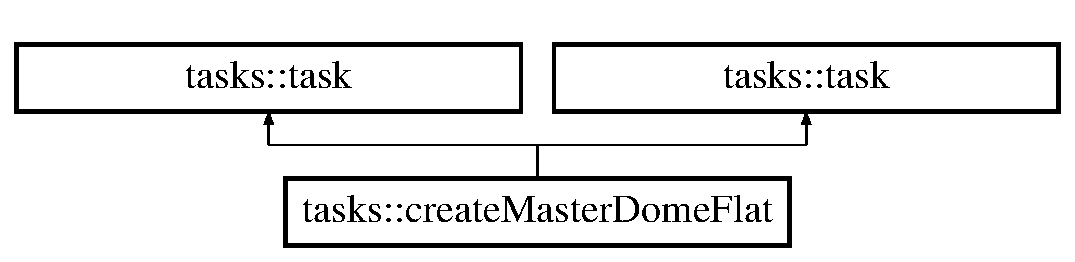
\includegraphics[height=2cm]{classtasks_1_1createMasterDomeFlat}
\end{center}
\end{figure}
\subsection*{Public Member Functions}
\begin{CompactItemize}
\item 
def \textbf{run}\label{classtasks_1_1createMasterDomeFlat_38c3a079e414119295ac097f7e448afa}

\item 
def \textbf{run}\label{classtasks_1_1createMasterDomeFlat_38c3a079e414119295ac097f7e448afa}

\end{CompactItemize}
\subsection*{Static Public Attributes}
\begin{CompactItemize}
\item 
string \textbf{name} = '{\bfcreate\-Master\-Dome\-Flat}'\label{classtasks_1_1createMasterDomeFlat_ff15c09eda22ae0f6e9023ba853fa3c5}

\item 
string \textbf{button\-Text} = 'Create Master Dome FLAT'\label{classtasks_1_1createMasterDomeFlat_1dbc69828d6b8c7191c1b36c5817ec05}

\end{CompactItemize}


\subsection{Detailed Description}


\footnotesize\begin{verbatim}Create a master Dome FLAT from the dome flatfield file list
\end{verbatim}
\normalsize
 



The documentation for this class was generated from the following files:\begin{CompactItemize}
\item 
old/PANICtool-1.0/tasks.py\item 
old/tasks.py\end{CompactItemize}
